\documentclass[conference]{IEEEtran}
\IEEEoverridecommandlockouts

% Citation management
\usepackage{cite}

% Text and list formatting
\usepackage{enumitem}
\usepackage{amsmath,amssymb,amsfonts}

% Algorithms (optional but common in empirical papers)
\usepackage{algorithm}
\usepackage{algorithmic}

% Graphics and visual elements
\usepackage{graphicx}
\usepackage{textcomp}
\usepackage{xcolor}
\usepackage{url}

% Figure and table enhancements
\usepackage{booktabs}
\usepackage{threeparttable}

% Diagrams (optional)
\usepackage{tikz}
\usetikzlibrary{arrows,positioning,fit,calc}

\begin{document}

\title{Closed-Loop Rolling Calibration for Forecast-Informed Reservoir Dispatch}

\author{%
\IEEEauthorblockN{Anonymous Authors}
\IEEEauthorblockA{Affiliation omitted}
}

\maketitle

\begin{IEEEkeywords}
reservoir inflow forecasting, rolling calibration, data assimilation, forecast-informed operation, model predictive control
\end{IEEEkeywords}

\begin{abstract}
Real-time reservoir dispatch depends critically on short-horizon inflow forecasts, yet nonstationarity and shifting operational constraints routinely erode calibration quality and degrade forecast-informed decision-making. We present a closed-loop framework that tightly couples rolling model calibration, uncertainty-aware probabilistic forecasting, and implementation feedback within a receding-horizon dispatch loop. At each decision cycle, model parameters are updated from the most recent observations; a probabilistic multi-step inflow forecast is generated; a scenario-based receding-horizon dispatch problem is solved; and realized outcomes are used to adaptively inflate forecast uncertainty when recent errors grow. We evaluate the framework on three reservoirs from the ResOpsUS historical operations dataset (daily storage, inflow, and outflow records spanning 1980--2020), using a strictly causal train/tune/test partition (1980--2010 / 2011--2014 / 2015--2020) and a 7-day forecast and dispatch horizon. Against a statically calibrated AR($p$) baseline, rolling calibration achieves comparable point-forecast skill while reducing mean CRPS by 16.3\% across reservoirs. In end-to-end dispatch simulation, closed-loop scenario MPC with feedback attains the lowest mean objective among all tested pipelines, reducing the mean operational objective by 0.33\% relative to a static open-loop deterministic MPC baseline; performance gains are reservoir-dependent, storage-bound violation rates remain comparable across methods, and the full decision cycle executes in approximately 20\,ms per day on CPU.
\end{abstract}

\section{Introduction}
Real-time reservoir operation relies on short-term inflow predictions to schedule releases
while satisfying safety constraints (e.g., flood control limits) and operational objectives
(e.g., hydropower generation, water supply). Classical reservoir operation studies emphasize
that optimal policies depend on both hydrologic dynamics and decision constraints
\cite{yeh1985reservoir,labadie2004optimal}.

Forecast errors and nonstationary conditions can induce systematic bias and drift in inflow
predictions. This drift raises operational risk. Yet the mapping from forecast skill to
operational value is complex and regime-dependent \cite{turner2017complex,milly2008stationarity}.

Rolling calibration and data assimilation provide a principled mechanism to adapt model
states and parameters online using incoming observations. Ensemble Kalman filter (EnKF)
variants have been widely used for dual state--parameter estimation and for improving
streamflow forecasting \cite{moradkhani2005dual,evensen2003ensemble,maxwell2018constraining,xiong2019identifying}.
The inflow forecasting literature also spans conceptual models, machine learning baselines,
and uncertainty-aware multi-step prediction
\cite{gragne2015improving,kratzert2018rainfall,kratzert2019learning,fan2023explainable}.

Forecast-informed reservoir operation (FIRO-style) and model predictive control (MPC)
approaches integrate forecasts into dispatch decisions, including uncertainty-aware
optimization using scenarios or ensembles \cite{liu2020reservoir,cestari2023scenario,mayne2000constrained,zarei2021machine}.
However, many existing workflows treat forecasting and dispatch as a sequential, largely
open-loop pipeline: forecasts are produced, an operating policy is computed, and the system
is executed with limited explicit coupling of implementation outcomes back into the next
forecast-and-dispatch cycle.

This paper proposes a closed-loop method that couples (i) rolling parameter calibration for
inflow forecasting, (ii) uncertainty-aware dispatch optimization, and (iii) implementation
feedback that updates the next decision cycle. We test whether making this coupling explicit
improves operational reliability under nonstationarity relative to open-loop baselines with
static calibration or without uncertainty propagation.

\begin{figure}[t]
\centering
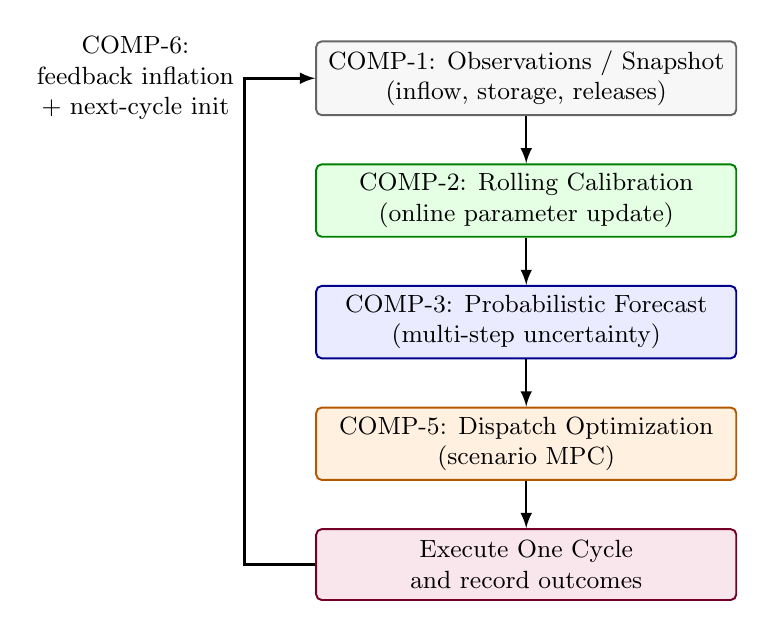
\begin{tikzpicture}[
  font=\small,
  block/.style={draw, rounded corners=2pt, align=center, minimum width=0.44\columnwidth, minimum height=9mm, line width=0.7pt},
  arrow/.style={->,>=latex, line width=0.9pt},
]

\node[block, fill=gray!6, draw=black!60] (obs) {COMP-1: Observations / Snapshot\\(inflow, storage, releases)};
\node[block, fill=green!10, draw=green!50!black, below=6mm of obs] (cal) {COMP-2: Rolling Calibration\\(online parameter update)};
\node[block, fill=blue!8, draw=blue!55!black, below=6mm of cal] (fcst) {COMP-3: Probabilistic Forecast\\(multi-step uncertainty)};
\node[block, fill=orange!12, draw=orange!70!black, below=6mm of fcst] (mpc) {COMP-5: Dispatch Optimization\\(scenario MPC)};
\node[block, fill=purple!10, draw=purple!60!black, below=6mm of mpc] (impl) {Execute One Cycle\\and record outcomes};

\draw[arrow] (obs) -- (cal);
\draw[arrow] (cal) -- (fcst);
\draw[arrow] (fcst) -- (mpc);
\draw[arrow] (mpc) -- (impl);

\draw[arrow] (impl.west) -- ++(-9mm,0) |- node[left,align=center,font=\small]{COMP-6:\\feedback inflation\\+ next-cycle init} (obs.west);

\end{tikzpicture}

\caption{Closed-loop coupling of rolling calibration, forecasting, dispatch, and implementation feedback.}
\label{fig:teaser}
\end{figure}

\subsection{Contributions}
\begin{itemize}[leftmargin=*]
\item[\textbf{C1}] \textbf{Closed-loop forecast--dispatch--feedback framework.}
We propose a unified closed-loop architecture that couples inflow forecasting, scenario-based dispatch optimization, and implementation feedback. Evaluated on ResOpsUS (3 reservoirs; test period 2015--2020), closed-loop scenario MPC with feedback reduces the mean operational objective by 0.33\% relative to a static open-loop deterministic MPC baseline, with reservoir-dependent gains and comparable storage-bound violation rates.

\item[\textbf{C2}] \textbf{Rolling calibration with quantified probabilistic skill.}
We instantiate online model updating via a lightweight AR($p$) inflow forecaster and assess both point and probabilistic forecast accuracy. Rolling calibration reduces mean CRPS by 16.3\% relative to a static AR($p$) baseline while leaving RMSE essentially unchanged, demonstrating that distributional accuracy improves without sacrificing point-forecast fidelity.

\item[\textbf{C3}] \textbf{Ablation of uncertainty propagation and feedback coupling.}
We systematically isolate the contribution of each pipeline component. Removing implementation feedback increases the operational objective by 0.16\%; replacing scenario MPC with deterministic dispatch increases it by 0.37\%.

\item[\textbf{C4}] \textbf{Stress tests and computational characterization.}
Scenario-based closed-loop optimization executes in approximately 20\,ms per daily cycle on CPU. The framework remains stable under synthetic regime shifts and sparse or delayed observations, with objective variation below 0.3\%, confirming practical robustness without incurring prohibitive computational overhead.
\end{itemize}

\section{Related Work}
We organize related work around the building blocks of a forecast--dispatch closed loop:
(i) rolling calibration, (ii) inflow forecasting with uncertainty, and (iii) forecast-informed
dispatch under constraints.

\begin{table}[t]
\centering
\caption{Taxonomy of building blocks for forecast-informed reservoir operation.}
\label{tab:taxonomy}
{\setlength{\tabcolsep}{3pt}\small
\begin{tabular}{p{0.42\columnwidth}p{0.52\columnwidth}}
\toprule
Building block & Representative references \\
\midrule
Rolling calibration / data assimilation & \cite{moradkhani2005dual,evensen2003ensemble,maxwell2018constraining,xiong2019identifying} \\
Multi-step inflow forecasting & \cite{gragne2015improving,kratzert2018rainfall,kratzert2019learning,fan2023explainable} \\
Forecast-informed operation and FIRO-style methods & \cite{yang2019real,zarei2021machine} \\
Uncertainty-aware dispatch (scenario MPC) & \cite{liu2020reservoir,cestari2023scenario,mayne2000constrained} \\
Forecast skill vs operational value & \cite{turner2017complex} \\
\bottomrule
\end{tabular}}
\end{table}

\subsection{Rolling Calibration and Data Assimilation}
EnKF-based dual estimation and related data assimilation methods update hidden states and
time-varying parameters online to reduce forecast errors \cite{moradkhani2005dual,evensen2003ensemble}.
Recent work also emphasizes the role of time-varying parameters under changing environments
and the need to constrain filtering behavior for stable performance \cite{xiong2019identifying,maxwell2018constraining}.

\subsection{Inflow Forecasting and Uncertainty}
Reservoir inflow forecasting spans complementary modeling frameworks and machine learning
baselines, increasingly with uncertainty quantification for multi-step prediction
\cite{gragne2015improving,kratzert2018rainfall,kratzert2019learning,fan2023explainable}.
For operational use, uncertainty calibration (e.g., CRPS and coverage) is often as important
as point-skill metrics \cite{gneiting2007strictly}.

\subsection{Forecast-Informed Reservoir Operation}
Forecast-informed operation integrates inflow predictions into dispatch policies, including
data-driven and recurrent-network approaches \cite{yang2019real,zarei2021machine,sushanth2023real}.
Yet improved forecast skill does not guarantee proportional operational gains, which motivates
evaluating both forecast metrics and operational outcomes \cite{turner2017complex}.
Recent studies also combine multi-step streamflow forecasts with multi-objective reservoir
operation and performance assessment \cite{guo2021ai}.

\subsection{Uncertainty-Aware Dispatch and MPC}
Scenario-based MPC provides a natural interface between probabilistic forecasts and
constraint-aware reservoir dispatch \cite{cestari2023scenario,mayne2000constrained}. Domain-specific
studies also show that forecast uncertainty varies across hydrologic periods, suggesting that
operating rules should account for these shifts \cite{liu2020reservoir}.
MPC-style operation has also been explored for flood mitigation in multi-reservoir settings
and for ensemble-forecast-driven multi-objective dam operation \cite{myolin2018flood,tanhapour2025development}.

\section{Method}
We describe a modular closed-loop framework that couples rolling forecast calibration with
forecast-informed dispatch. The design follows a receding-horizon decision cycle and can wrap
either conceptual or data-driven inflow models. We emphasize the coupling logic rather than
introducing a new forecasting architecture.

\subsection{Problem Setup}
Let $k$ index decision cycles with control interval $\Delta t$ (e.g., hourly or daily). At the
beginning of cycle $k$, the operator observes a state snapshot $x_k$ (e.g., storage, recent
inflows, releases, and constraint indicators) and optionally exogenous covariates (e.g.,
meteorological forcings). The task is to compute a release plan
over a finite horizon $H$ while satisfying operational constraints (e.g., storage bounds,
release limits, and safety constraints) \cite{yeh1985reservoir,labadie2004optimal}.

We distinguish between:
\begin{itemize}[leftmargin=*]
\item \textbf{Forecasting}: generate a probabilistic inflow forecast $\hat{q}_{k+1:k+H}$.
\item \textbf{Dispatch}: compute releases $r_{k:k+H}$ (or a subset such as $r_k$) using the forecast.
\item \textbf{Implementation}: apply the release for one cycle, observe outcomes, and feed them back.
\end{itemize}

\paragraph{Notation}
We use $q_t$ for realized inflow at day $t$, $\hat{q}_{t+1:t+H}$ for a horizon-$H$ inflow
forecast, $r_t$ for the implemented release, and $s_t$ for storage. Subscripts $k$ and $t$
both index decision cycles (we use $t$ for day-indexed equations consistent with the
implementation).

\subsection{Approach Overview}
The framework consists of six components:
(i) observation/state snapshot, (ii) rolling parameter calibration, (iii) probabilistic inflow
forecasting, (iv) scenario generation, (v) scenario-based MPC dispatch, and (vi) an
implementation-feedback loop orchestrator.

\paragraph{Rolling parameter calibration}
We update model state and parameters online using incoming observations, motivated by EnKF
dual-estimation and constrained filtering for stable forecasting
\cite{moradkhani2005dual,evensen2003ensemble,maxwell2018constraining,xiong2019identifying}.
The calibration step outputs an updated parameter set $\theta_k$ and (optionally) an updated
state estimate used by the forecaster.

\paragraph{Probabilistic inflow forecasting and scenario generation}
Given $\theta_k$ and the current state, the forecaster produces an ensemble (or quantiles) of
inflow trajectories. Scenarios are passed to the dispatcher either directly (ensemble-as-scenarios)
or via a lightweight scenario generator. We evaluate uncertainty calibration using proper
scoring rules such as CRPS \cite{gneiting2007strictly}.

\paragraph{Uncertainty-aware dispatch (scenario MPC)}
The dispatcher solves a receding-horizon optimization that accounts for constraints and forecast
uncertainty. Scenario-based MPC provides a natural interface for this step
\cite{cestari2023scenario,mayne2000constrained,raso2017combining}.

\begin{figure}[t]
\centering
\resizebox{\columnwidth}{!}{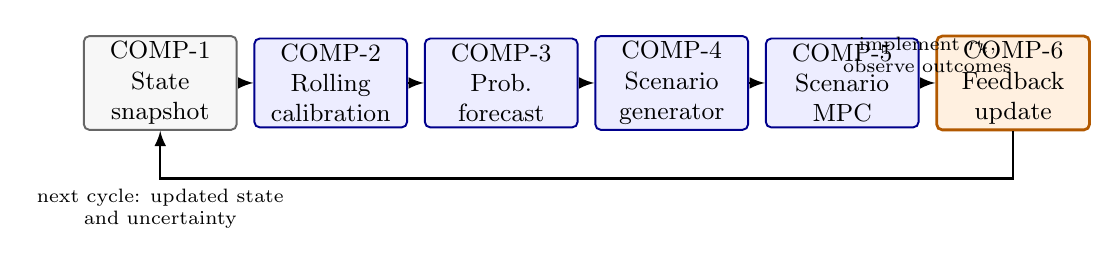
\begin{tikzpicture}[
  font=\small,
  block/.style={draw, rounded corners=2pt, align=center, text width=18mm, inner sep=2pt, minimum height=9mm, line width=0.7pt, fill=gray!6, draw=black!60},
  stage/.style={block, fill=blue!7, draw=blue!55!black},
  novel/.style={block, fill=orange!12, draw=orange!70!black, line width=1.0pt},
  arrow/.style={->,>=latex, line width=0.9pt},
]

\node[block] (snap) {COMP-1\\State\\snapshot};
\node[stage, right=2mm of snap] (cal) {COMP-2\\Rolling\\calibration};
\node[stage, right=2mm of cal] (fcst) {COMP-3\\Prob.\\forecast};
\node[stage, right=2mm of fcst] (scen) {COMP-4\\Scenario\\generator};
\node[stage, right=2mm of scen] (opt) {COMP-5\\Scenario\\MPC};
\node[novel, right=2mm of opt] (fb) {COMP-6\\Feedback\\update};

\draw[arrow] (snap) -- (cal);
\draw[arrow] (cal) -- (fcst);
\draw[arrow] (fcst) -- (scen);
\draw[arrow] (scen) -- (opt);
\draw[arrow] (opt) -- node[above,align=center,font=\scriptsize]{implement $r_k$,\\observe outcomes} (fb);

\draw[arrow] (fb.south) |- ++(0,-6mm) -| node[below,align=center,font=\scriptsize]{next cycle: updated state\\and uncertainty} (snap.south);

\end{tikzpicture}
}
\caption{Method pipeline components. After scenario MPC selects the first control action, realized outcomes enter COMP-6, which updates next-cycle state and uncertainty information for the following decision cycle.}
\label{fig:pipeline}
\end{figure}

\paragraph{Implementation feedback and closed-loop coupling}
After executing the first control action (or first segment) of the plan, we observe realized
inflow, state transitions, and constraint outcomes. These signals are injected into the next
cycle. This closes the loop between forecast, dispatch, and implementation, enabling ablations
that isolate the value of rolling calibration, uncertainty propagation, and feedback coupling.

\subsection{Closed-Loop Cycle Algorithm}
\begin{algorithm}[t]
\caption{Closed-loop forecast--dispatch--implementation coupling (per cycle $k$).}
\begin{algorithmic}[1]
\STATE Observe state snapshot $x_k$ and recent operations/measurements.
\STATE Update forecast-model state/parameters via rolling calibration: $\theta_k \leftarrow \mathrm{Calibrate}(x_k)$.
\STATE Generate probabilistic inflow forecast over horizon $H$: $\hat{q}_{k+1:k+H} \leftarrow \mathrm{Forecast}(x_k,\theta_k)$.
\STATE Convert forecasts to scenarios (optional): $\mathcal{S}_k \leftarrow \mathrm{Scenarios}(\hat{q}_{k+1:k+H})$.
\STATE Solve uncertainty-aware dispatch (scenario MPC): $r_{k:k+H} \leftarrow \mathrm{Dispatch}(x_k,\mathcal{S}_k)$.
\STATE Implement $r_k$ for one cycle; observe realized outcomes and constraint status.
\STATE Advance to cycle $k{+}1$ using implementation feedback.
\end{algorithmic}
\end{algorithm}

\subsection{Rolling Calibration via Recursive Least Squares}
For clarity and reproducibility, we instantiate the rolling-calibration module (COMP-2) using
a lightweight autoregressive forecaster with online parameter updates. Let $q_t$ denote daily
inflow at day $t$. We use an AR($p$) model with intercept:
\begin{equation}
q_t = \beta_0 + \sum_{i=1}^{p} \beta_i q_{t-i} + \varepsilon_t, \quad \varepsilon_t \sim \mathcal{N}(0,\sigma_t^2).
\end{equation}
Define the feature vector $\phi_t = [1, q_{t-1}, \dots, q_{t-p}]^\top$ and parameter vector
$\theta_t = [\beta_0, \beta_1, \dots, \beta_p]^\top$. Rolling calibration updates $\theta_t$
using recursive least squares (RLS) with exponential forgetting factor $\lambda$:
\begin{align}
K_t &= \frac{P_{t-1}\phi_t}{\lambda + \phi_t^\top P_{t-1}\phi_t}, \\
\theta_t &= \theta_{t-1} + K_t\left(q_t - \phi_t^\top\theta_{t-1}\right), \\
P_t &= \frac{1}{\lambda}\left(P_{t-1} - K_t\phi_t^\top P_{t-1}\right).
\end{align}
We initialize $\theta$ using a static ridge fit on the training period and warm-start RLS
through the tuning period so the test period begins from a stable state.
We track predictive uncertainty with an EWMA variance estimator:
\begin{equation}
\sigma_t^2 = \alpha\sigma_{t-1}^2 + (1-\alpha)\left(q_t - \phi_t^\top\theta_{t-1}\right)^2,
\end{equation}
where $\alpha \in [0,1)$ controls adaptation speed.

\subsection{Probabilistic Forecast and Scenario Generation}
Given $\theta_t$ and history up to day $t{-}1$, we produce a multi-step mean forecast
$\mu_{t+1:t+H}$ by iterating the AR recursion forward.
We approximate the $h$-step predictive standard deviation by $\sigma_t\sqrt{h}$, reflecting
accumulation of one-step residual uncertainty over the horizon.
For scenario MPC, we generate $|\mathcal{S}|$ inflow scenarios by sampling i.i.d.\ standard
Gaussians $z^{(s)}_h$ and forming:
\begin{equation}
q^{(s)}_{t+h} = \max\left(0,\,\mu_{t+h} + \gamma_t\,\sigma_t\sqrt{h}\,z^{(s)}_h\right),
\end{equation}
where $\gamma_t$ is an optional feedback inflation factor (COMP-6). Deterministic dispatch is
recovered by setting $|\mathcal{S}|{=}1$ and $z^{(1)}_h{=}0$.

\subsection{Scenario MPC Dispatch Objective}
For each scenario, we simulate the storage dynamics over the horizon and solve a
receding-horizon optimization for the release sequence. The stage cost is a quadratic proxy
that trades off target tracking, actuation effort, smoothness, and soft penalties for storage
violations:
\begin{equation}
\ell(s_{t+1}, r_t, r_{t-1}) =
\begin{aligned}[t]
& w_s(s_{t+1}-s^\star)^2 + w_r r_t^2 \\
& {}+ w_{\Delta r}(r_t-r_{t-1})^2 + w_v\,\mathrm{Viol}(s_{t+1}).
\end{aligned}
\end{equation}
We define $\mathrm{Viol}(s) = \max(0, s-\bar{s})^2 + \max(0, \underline{s}-s)^2$ and constrain
releases to $r_t \in [\underline{r}, \bar{r}]$. The MPC implements only the first release each
cycle, then replans at the next cycle using updated observations and calibrated parameters.

\subsection{Implementation Feedback via Adaptive Inflation}
Closed-loop coupling (COMP-6) modifies the next-cycle scenario spread based on recent realized
errors. We maintain a fast EWMA of squared one-step prediction errors $e_t^2$ and compute:
\begin{equation}
\gamma_t = \mathrm{clip}\left(\sqrt{\frac{\mathrm{EWMA}(e_t^2)}{\sigma_t^2}},\, 1,\, \gamma_{\max}\right),
\end{equation}
so scenario dispersion increases when short-term errors spike. This is a simple, implementable
feedback mechanism that can be ablated independently from rolling calibration and uncertainty
propagation.

\section{Experimental Setup}

\subsection{Datasets and Preprocessing}
We evaluate on ResOpsUS, a dataset of historical reservoir operations in the contiguous United
States \cite{steyaert2022resopsus}. Reservoir metadata are linked to global dam inventories
such as GRanD \cite{lehner2011high}. We select three reservoirs with complete daily records
from 1980-01-01 to 2020-12-31: Glen Canyon (DAM\_ID 597, AZ), Flaming Gorge (DAM\_ID 451, UT),
and Navajo (DAM\_ID 601, NM). Each day includes storage (MCM), inflow (m$^3$/s), and outflow
(m$^3$/s).

We use a strictly chronological split: training (1980--2010), tuning (2011--2014), and test
(2015--2020), reflecting nonstationarity and regime shifts \cite{milly2008stationarity}. All
rolling calibration and dispatch decisions in the test period are strictly causal: the
decision for day $t$ uses information available up to day $t{-}1$.
Figure~\ref{fig:inflow_timeseries} visualizes the daily inflow series and split boundaries for
the three case studies.

\begin{figure*}[t]
\centering
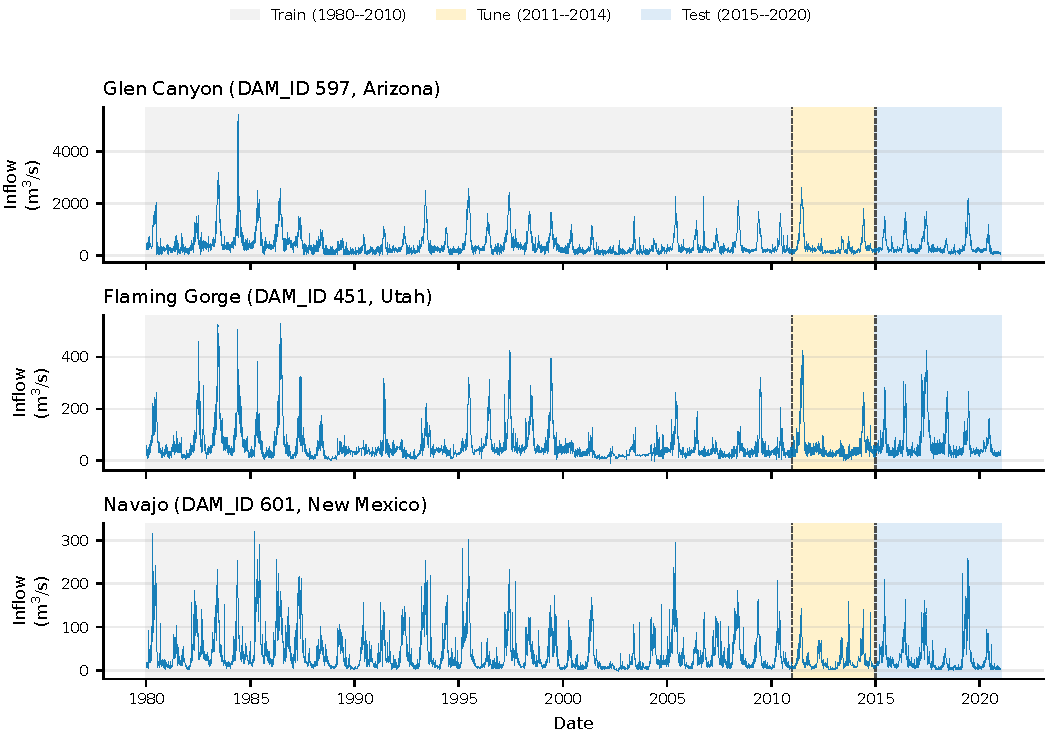
\includegraphics[width=\textwidth]{figures/inflow_timeseries_splits.pdf}
\caption{Daily inflow time series for the three ResOpsUS reservoirs (1980--2020) with chronological splits (train/tune/test).}
\label{fig:inflow_timeseries}
\end{figure*}

\subsection{Closed-Loop Simulator and Constraints}
Closed-loop operational performance is evaluated by simulating the reservoir mass balance and
operational constraints. Following standard reservoir optimization formulations
\cite{yeh1985reservoir,labadie2004optimal}, we use a discrete-time storage update:
\begin{equation}
s_{k+1} = s_k + (q_k - r_k - \mathrm{spill}_k)\Delta t,
\end{equation}
where $s_k$ is storage, $q_k$ is (realized) inflow, and $r_k$ is the implemented release.
Constraints include storage bounds, release bounds, and optional ramping/operational constraints.
For the ResOpsUS case studies, storage and release bounds are derived from training-period
quantiles. Over multi-year rollouts, unmodeled losses (e.g., evaporation or spill not available
in the time series) can cause drift. We estimate an aggregate daily loss term from training
mass-balance residuals and treat it as constant during simulation.
The dispatch module is solved in a receding-horizon model predictive control (MPC) manner
\cite{mayne2000constrained}. Uncertainty-aware variants use scenarios generated from forecast
distributions or ensembles \cite{liu2020reservoir,cestari2023scenario}.

\subsection{Rolling-Calibration Evaluation Protocol}
We report both forecast skill and closed-loop operational value, since improvements in forecast
accuracy do not necessarily translate into proportional operational gains \cite{turner2017complex}.
For each decision cycle in the test period, we:
\begin{itemize}[leftmargin=*]
\item update forecast-model parameters using a rolling window of the most recent $W$ observations,
using either EnKF-style dual state--parameter estimation when applicable
\cite{evensen2003ensemble,moradkhani2005dual} or a constrained sliding-window optimizer;
\item generate an inflow forecast over horizon $H$ (optionally probabilistic), and map uncertainty
to a scenario set for the dispatch optimizer;
\item solve the dispatch problem over horizon $H$ and implement only the first control action;
\item advance the simulator using realized inflows, and record objective and constraint outcomes.
\end{itemize}
To reduce identifiability artifacts in online estimation, time-varying parameters are regularized
and bounded, and we monitor stability diagnostics during rollouts
\cite{maxwell2018constraining,xiong2019identifying}.

\subsection{Baselines}
Baselines are grouped by forecasting and operation components. The main comparisons follow a
controlled-ablation philosophy:
\begin{itemize}[leftmargin=*]
\item Forecast baselines: persistence, seasonal climatology (day-of-year mean), a statically calibrated AR($p$)
time-series model, and an ML-LSTM sequence model \cite{kratzert2018rainfall,kratzert2019learning}. Our forecaster
uses the same AR($p$) structure with online rolling calibration and probabilistic error modeling.
\item Operation baselines: static-calibration open-loop deterministic MPC, rolling-calibration open-loop deterministic MPC,
rolling-calibration open-loop scenario MPC, and the proposed rolling-calibration closed-loop scenario MPC with feedback.
\end{itemize}

\subsection{Metrics}
We report both forecast skill and operational performance metrics:
\begin{itemize}[leftmargin=*]
\item Forecast metrics: RMSE/MAE, Nash--Sutcliffe efficiency (NSE) \cite{nash1970river}, and uncertainty metrics such as
CRPS and coverage \cite{gneiting2007strictly}.
\item Operational metrics: constraint-violation rate and objective value, plus reliability/resiliency/vulnerability-style
criteria when appropriate \cite{hashimoto1982reliability}.
\end{itemize}

\subsection{Implementation Details and Reproducibility}
Unless otherwise stated, all methods are evaluated at the same decision cycle $\Delta t$ and horizon $H$ under identical
data splits and pre-processing. For stochastic baselines (e.g., neural forecasting models), we report results across
multiple random seeds and document training and early-stopping criteria on the tuning period. For each run, we report
the rolling calibration configuration (window length $W$, update frequency, and any regularization), the scenario
generation settings (scenario count and sampling scheme), and the dispatch solver settings (tolerances and maximum
iterations). We also report wall-clock runtime per decision cycle to assess operational feasibility.

\begin{table}[t]
\centering
\caption{Experimental setup summary (ResOpsUS case studies).}
\label{tab:setup}
{\setlength{\tabcolsep}{3pt}\small
\begin{tabular}{p{0.31\columnwidth}p{0.63\columnwidth}}
\toprule
Item & Specification \\
\midrule
Case study & ResOpsUS (3 reservoirs; daily 1980--2020; test 2015--2020) \\
Decision cycle / horizon & $\Delta t$ = 1 day; $H$ = 7 days \\
Rolling calibration & AR(3) recursive least squares; forgetting factor $\lambda$=0.999; update freq.=1/day \\
Uncertainty propagation & Gaussian residual model; EWMA variance ($\alpha$=0.98); $|\mathcal{S}|$=20 scenarios; feedback inflation max=3.0 \\
Bounds & storage/release bounds from training 5\%--95\% quantiles \\
Forecast metrics & RMSE, MAE, NSE; CRPS; 80\% coverage \\
Operational metrics & storage-bound violation rate; objective; reliability/vulnerability \\
\bottomrule
\end{tabular}}
\end{table}

\section{Results}
We report forecast skill and operational value on the ResOpsUS case studies. Unless stated
otherwise, table entries are mean$\pm$std across the three reservoirs in the test period
(2015--2020).

\subsection{Forecast Skill}
We report multi-step inflow forecast skill over the operational horizon using point metrics
(RMSE/MAE and NSE \cite{nash1970river}). When probabilistic forecasts are available, we also
report proper scoring rules such as CRPS and empirical coverage \cite{gneiting2007strictly}. To
reflect nonstationarity, we stratify test performance by hydrologic regime when possible
\cite{milly2008stationarity}.

\begin{table}[t]
\centering
\caption{Forecast main results on ResOpsUS (test 2015--2020; $H$=7 days).}
\label{tab:forecast_results}
{\setlength{\tabcolsep}{2pt}\scriptsize
\resizebox{\columnwidth}{!}{%
\begin{tabular}{p{0.34\columnwidth}cccc}
\toprule
Method & RMSE & NSE & CRPS & Cov. \\
\midrule
Persistence & 54.44$\pm$55.82 & 0.836$\pm$0.044 & 34.87$\pm$40.41 & 0.940$\pm$0.036 \\
Climatology & 102.81$\pm$110.70 & 0.473$\pm$0.088 & 92.66$\pm$109.10 & 0.979$\pm$0.013 \\
AR(p) static & 53.33$\pm$55.90 & 0.848$\pm$0.039 & 31.11$\pm$35.21 & 0.937$\pm$0.026 \\
ML-LSTM & 57.63$\pm$62.10 & 0.834$\pm$0.031 & 28.89$\pm$31.93 & 0.901$\pm$0.019 \\
Rolling AR(p) (ours) & 53.40$\pm$55.45 & 0.845$\pm$0.044 & 26.03$\pm$27.79 & 0.915$\pm$0.020 \\
\bottomrule
\end{tabular}}
}

\end{table}

\begin{figure}[t]
\centering
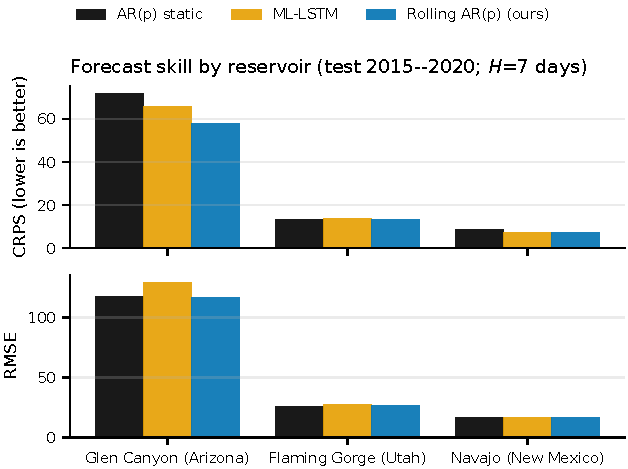
\includegraphics[width=\columnwidth]{figures/forecast_skill_by_dam.pdf}
\caption{Forecast skill broken down by reservoir for key methods (test 2015--2020; $H$=7 days).}
\label{fig:forecast_skill_by_dam}
\end{figure}

\begin{figure}[t]
\centering
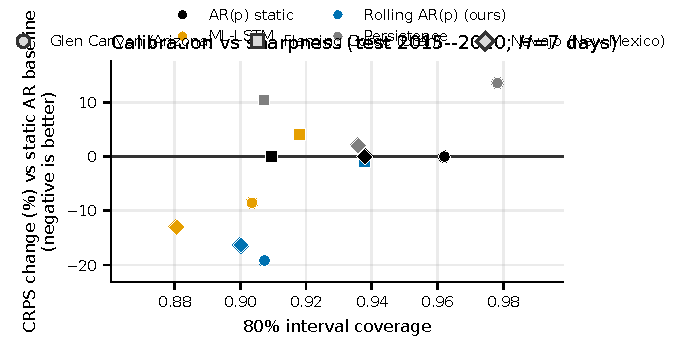
\includegraphics[width=\columnwidth]{figures/forecast_calibration_tradeoff.pdf}
\caption{Calibration vs sharpness tradeoff for key forecasters (test 2015--2020; $H$=7 days). X-axis: nominal 80\% interval coverage. Y-axis: CRPS change (\%) relative to the static AR baseline for the same reservoir (negative is better). Marker shape indicates reservoir; dashed vertical line marks the nominal 0.8 coverage.}
\label{fig:forecast_calibration_tradeoff}
\end{figure}

Rolling calibration primarily improves probabilistic calibration. Relative to the static
AR($p$) baseline, mean CRPS decreases from 31.11 to 26.03 (16.3\%). RMSE remains essentially
unchanged (53.33 to 53.40; $<0.2\%$ increase), and NSE shifts from 0.848 to 0.845. Coverage for
the nominal 80\% interval decreases from 0.937 to 0.915, indicating less conservative
uncertainty while improving CRPS. Figure~\ref{fig:forecast_calibration_tradeoff} shows that
all evaluated forecasters remain conservative (coverage $>$ 0.8), but rolling calibration
reduces over-coverage while lowering CRPS. Figure~\ref{fig:forecast_skill_by_dam} shows that this
improvement is heterogeneous across reservoirs: relative to the static AR($p$) baseline, CRPS
decreases by 0.9\% (Flaming Gorge), 19.2\% (Glen Canyon), and 16.3\% (Navajo).

\subsection{Operational Main Results}
We report end-to-end closed-loop performance under receding-horizon dispatch
\cite{mayne2000constrained}. We include both deterministic and scenario-based variants
\cite{liu2020reservoir,cestari2023scenario}. We focus on constraint violations, objective
value, and reliability-style criteria \cite{hashimoto1982reliability}. We analyze operational
value separately from forecast skill \cite{turner2017complex}.
Closed-loop scenario MPC with feedback achieves the lowest average objective among the tested
pipelines, with similar storage-bound violation rates.

\begin{table}[t]
\centering
\caption{Operational main results on ResOpsUS (test 2015--2020). Objective is reported in $\times 10^6$ cost units (lower is better).}
\label{tab:main_results}
{\setlength{\tabcolsep}{2pt}\scriptsize
\resizebox{\columnwidth}{!}{%
\begin{tabular}{p{0.34\columnwidth}ccp{0.24\columnwidth}}
\toprule
Method & Viol. & Obj. ($\times10^6$) & Notes \\
\midrule
Static det. MPC (baseline) & 0.032$\pm$0.056 & 9.20$\pm$8.28 & open-loop + static params \\
Rolling det. MPC & 0.032$\pm$0.056 & 9.21$\pm$8.28 & isolates rolling calibration \\
Rolling scenario MPC & 0.032$\pm$0.056 & 9.19$\pm$8.26 & isolates uncertainty-aware dispatch \\
Closed-loop scenario MPC (ours) & 0.032$\pm$0.056 & 9.17$\pm$8.24 & closed-loop coupling \\
\bottomrule
\end{tabular}}
}

\end{table}

\begin{figure}[t]
\centering
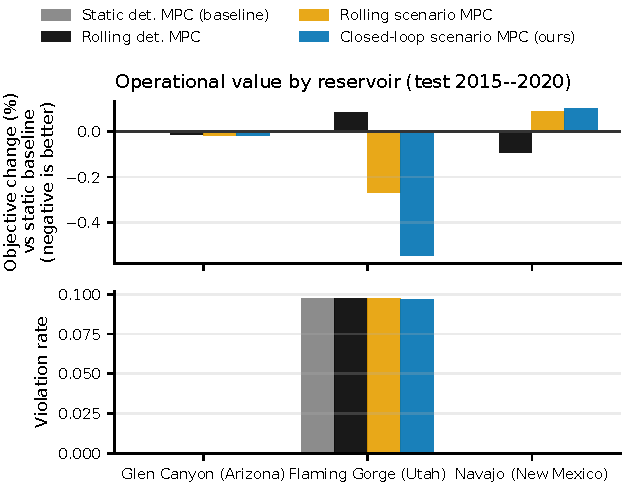
\includegraphics[width=\columnwidth]{figures/ops_by_dam.pdf}
\caption{Operational objective change (relative to static open-loop deterministic MPC) and storage-bound violation rate, broken down by reservoir (test 2015--2020). Objective change is reported as a percent difference; negative values indicate lower cost (better).}
\label{fig:ops_by_dam}
\end{figure}

Compared with the static open-loop deterministic baseline, closed-loop scenario MPC with
feedback reduces the mean operational objective from 9.20 to 9.17$\times 10^6$ (0.33\%). The
mean violation rate is similar (0.0324 vs.\ 0.0322). Violations are concentrated in Flaming
Gorge, while the other two reservoirs have zero violations across all tested pipelines
(Figure~\ref{fig:ops_by_dam}). The objective change is reservoir-dependent: relative to the
static baseline, our method changes objective by $-0.55\%$ (Flaming Gorge), $-0.02\%$ (Glen
Canyon), and $+0.10\%$ (Navajo).

\subsection{Ablation Studies}
We ablate the core coupling components to isolate their marginal value (EXP-ABL-*):
rolling calibration, uncertainty propagation (scenario-based dispatch), and implementation feedback.

\begin{table}[t]
\centering
\caption{Ablation results on ResOpsUS (test 2015--2020). Objective is reported in $\times 10^6$ cost units (lower is better).}
\label{tab:ablation_results}
{\setlength{\tabcolsep}{2pt}\scriptsize
\resizebox{\columnwidth}{!}{%
\begin{tabular}{p{0.34\columnwidth}ccp{0.24\columnwidth}}
\toprule
Method & Viol. & Obj. ($\times10^6$) & Notes \\
\midrule
Full closed-loop method & 0.032$\pm$0.056 & 9.17$\pm$8.24 & reference \\
w/o rolling calibration (static params) & 0.032$\pm$0.056 & 9.17$\pm$8.23 & ablate COMP-2 \\
w/o implementation feedback (open loop) & 0.032$\pm$0.056 & 9.19$\pm$8.26 & ablate COMP-6 \\
Deterministic dispatch (no scenarios) & 0.032$\pm$0.056 & 9.21$\pm$8.28 & ablate uncertainty propagation \\
Point forecast only (no UQ) & 0.032$\pm$0.056 & 9.21$\pm$8.28 & remove probabilistic forecasts \\
\bottomrule
\end{tabular}}
}

\end{table}

\begin{figure}[t]
\centering
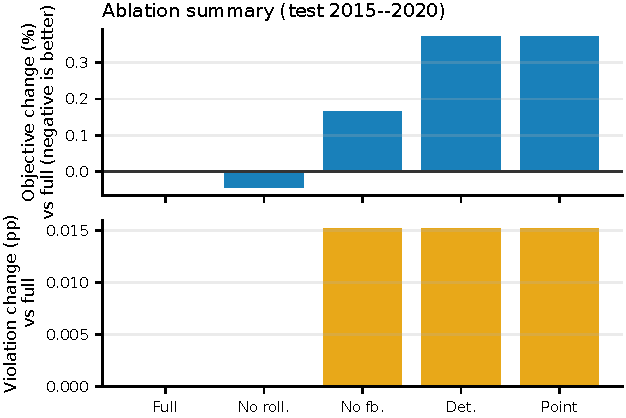
\includegraphics[width=\columnwidth]{figures/ablation_summary.pdf}
\caption{Ablation summary relative to the full closed-loop method (test 2015--2020). Top: objective change (\%) vs full; negative indicates lower cost (better). Bottom: storage-bound violation-rate change in percentage points (pp) vs full.}
\label{fig:ablation_summary}
\end{figure}

The ablation results attribute most objective gains to uncertainty propagation and feedback
(Figure~\ref{fig:ablation_summary}).
Relative to the full method (9.17$\times 10^6$), removing feedback increases the objective to
9.19$\times 10^6$ (+0.16\%). Replacing scenario MPC with deterministic dispatch (or using point
forecasts only) increases it to 9.21$\times 10^6$ (+0.37\%). In this proxy objective, removing
rolling calibration changes the objective by less than 0.05\%.

\subsection{Error Analysis / Robustness}
We evaluate robustness to synthetic regime shifts (multiplicative inflow scaling) and to
sparse/delayed observations used for rolling calibration (EXP-ROB-*). Stress tests are
motivated by known failure modes in online data assimilation and calibration
\cite{evensen2003ensemble,moradkhani2005dual,maxwell2018constraining}.

\begin{table}[t]
\centering
\caption{Robustness stress tests (excerpt). Objective is reported in $\times 10^6$ cost units (lower is better). Full results are provided in the accompanying artifacts.}
\label{tab:robustness}
{\setlength{\tabcolsep}{2pt}\scriptsize
\resizebox{\columnwidth}{!}{%
\begin{tabular}{p{0.26\columnwidth}p{0.22\columnwidth}p{0.30\columnwidth}cc}
\toprule
Stress & Severity & Method & Viol. & Obj. ($\times10^6$) \\
\midrule
inflow\_scale & 0.8 & Static det. MPC (baseline) & 0.014 & 7.74 \\
inflow\_scale & 0.8 & Rolling det. MPC & 0.014 & 7.74 \\
inflow\_scale & 0.8 & Closed-loop scenario MPC (ours) & 0.014 & 7.74 \\
inflow\_scale & 0.9 & Static det. MPC (baseline) & 0.023 & 6.87 \\
inflow\_scale & 0.9 & Rolling det. MPC & 0.023 & 6.88 \\
inflow\_scale & 0.9 & Closed-loop scenario MPC (ours) & 0.023 & 6.87 \\
inflow\_scale & 1.0 & Static det. MPC (baseline) & 0.032 & 9.20 \\
inflow\_scale & 1.0 & Rolling det. MPC & 0.032 & 9.21 \\
inflow\_scale & 1.0 & Closed-loop scenario MPC (ours) & 0.032 & 9.17 \\
inflow\_scale & 1.1 & Static det. MPC (baseline) & 0.042 & 15.15 \\
inflow\_scale & 1.1 & Rolling det. MPC & 0.042 & 15.16 \\
inflow\_scale & 1.1 & Closed-loop scenario MPC (ours) & 0.042 & 15.13 \\
inflow\_scale & 1.2 & Static det. MPC (baseline) & 0.068 & 25.73 \\
inflow\_scale & 1.2 & Rolling det. MPC & 0.068 & 25.74 \\
inflow\_scale & 1.2 & Closed-loop scenario MPC (ours) & 0.068 & 25.64 \\
obs\_sparse\_delay & miss=0.0,delay=0 & Closed-loop (ours) & 0.032 & 9.18 \\
obs\_sparse\_delay & miss=0.0,delay=1 & Closed-loop (ours) & 0.032 & 9.19 \\
obs\_sparse\_delay & miss=0.0,delay=3 & Closed-loop (ours) & 0.032 & 9.19 \\
\bottomrule
\end{tabular}}
}

\end{table}

\begin{figure}[t]
\centering
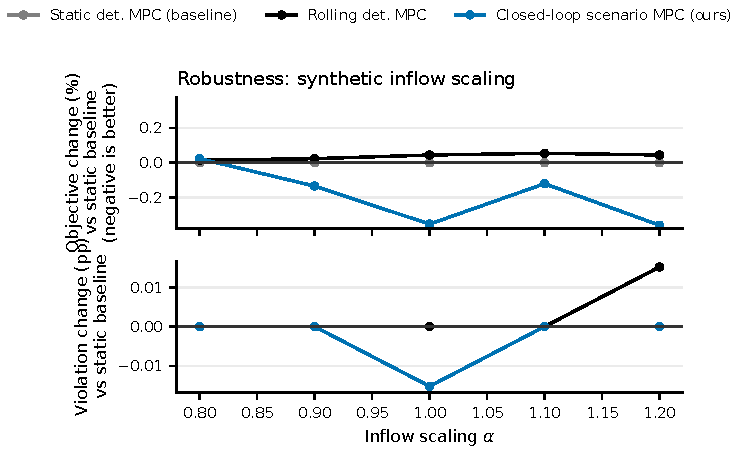
\includegraphics[width=\columnwidth]{figures/robustness_inflow_scale.pdf}
\caption{Robustness to a synthetic regime shift induced by multiplicative inflow scaling ($\alpha$). Top: objective change (\%) vs static open-loop deterministic MPC (baseline) at each $\alpha$; negative indicates lower cost (better). Bottom: storage-bound violation-rate change in percentage points (pp) vs baseline.}
\label{fig:robustness_inflow_scale}
\end{figure}

\begin{figure}[t]
\centering
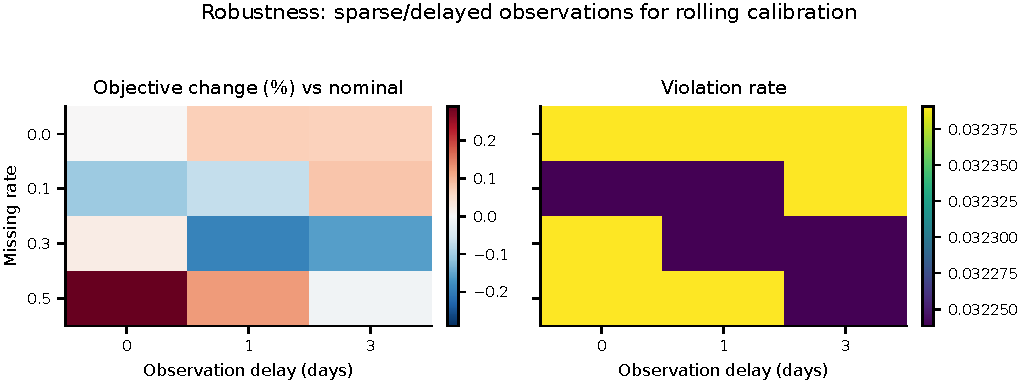
\includegraphics[width=\columnwidth]{figures/robustness_obs_sparse_delay.pdf}
\caption{Robustness of closed-loop rolling calibration to sparse and delayed observations. Left: objective change relative to nominal ($\mathrm{miss}=0$, delay=0); negative indicates lower cost (better). Right: violation rate.}
\label{fig:robustness_obs_sparse_delay}
\end{figure}

\paragraph{Inflow regime shift.}
Under severe inflow scaling ($\alpha$=1.2), closed-loop feedback reduces the mean objective
from 25.73 to 25.64$\times 10^6$ (0.36\%) while maintaining essentially identical violation
rates (0.0677). This result suggests that the feedback mechanism can provide a modest
advantage over the open-loop baseline under a substantial shift in inflow magnitude.

\paragraph{Sparse and delayed observations.}
When rolling calibration operates under degraded observational conditions---up to 50\%
missing measurements and a 3-day reporting delay---the mean objective varies by less than
0.3\% relative to the nominal setting, and violation rates remain tightly bounded within
[0.03224, 0.03239]. This insensitivity indicates that the calibration loop can tolerate
realistic monitoring imperfections without large operational degradation.

\subsection{Efficiency}
We measure per-cycle runtime for calibration and dispatch to assess feasibility at a daily
decision cadence (EXP-EFF-RUNTIME).

\begin{table}[t]
\centering
\caption{Efficiency comparison (mean per-cycle runtime on CPU).}
\label{tab:efficiency}
{\setlength{\tabcolsep}{2pt}\scriptsize
\resizebox{\columnwidth}{!}{%
\begin{tabular}{p{0.44\columnwidth}ccc}
\toprule
Method & Calib (s) & Dispatch (s) & Total (s) \\
\midrule
Static det. MPC (baseline) & 0.000 & 0.003 & 0.003 \\
Rolling scenario MPC & 0.000 & 0.020 & 0.020 \\
Closed-loop scenario MPC (ours) & 0.000 & 0.020 & 0.020 \\
\bottomrule
\end{tabular}}
}

\end{table}

\begin{figure}[t]
\centering
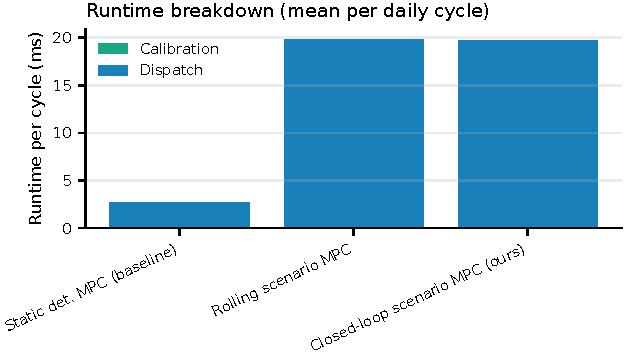
\includegraphics[width=\columnwidth]{figures/runtime_breakdown.pdf}
\caption{Runtime breakdown per daily cycle into rolling-calibration and dispatch components (mean over reservoirs).}
\label{fig:runtime_breakdown}
\end{figure}

\begin{figure}[t]
\centering
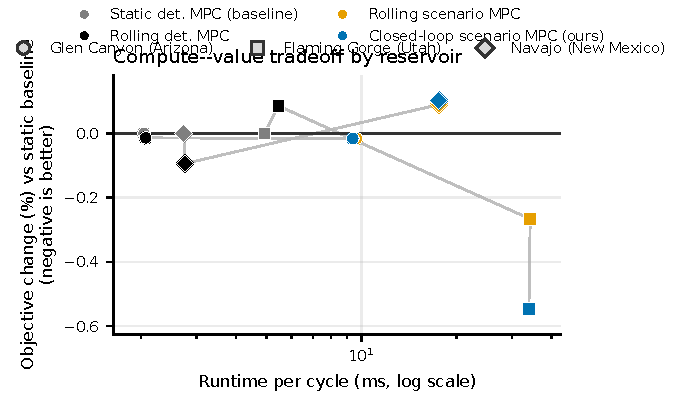
\includegraphics[width=\columnwidth]{figures/runtime_value_tradeoff.pdf}
\caption{Compute--value tradeoff across pipelines (test 2015--2020). Each point corresponds to one reservoir-method pair; color indicates method, marker shape indicates reservoir, and gray polylines connect the increasing-complexity pipeline within each reservoir. Runtime is shown on a log scale, and objective change is reported relative to the static deterministic baseline.}
\label{fig:runtime_value_tradeoff}
\end{figure}

Scenario-based MPC requires about 20\,ms per daily cycle on CPU, compared with about 3.3\,ms
for the deterministic baseline. Rolling-calibration updates contribute roughly 0.04\,ms per
cycle, so runtime is dominated by the dispatch optimization.

\section{Discussion}
\subsection{Forecast Skill vs.\ Operational Value}
Rolling calibration leaves point-skill nearly unchanged but improves probabilistic calibration
(CRPS). This pattern is consistent with the idea that operational value depends on the
decision context, not only on point accuracy \cite{turner2017complex}. In our proxy objective,
closed-loop scenario MPC yields a modest average improvement (0.33\%), while constraint
violation rates remain comparable across pipelines. The per-reservoir breakdown
(Figures~\ref{fig:forecast_skill_by_dam} and \ref{fig:ops_by_dam}) suggests that the operational
gain is driven primarily by a subset of reservoirs and periods where uncertainty interacts
with storage bounds. Figure~\ref{fig:forecast_calibration_tradeoff} further indicates that all
evaluated forecasters remain conservative (coverage $>$ 0.8), and that rolling calibration
reduces this over-coverage while lowering CRPS.

\subsection{Role of Uncertainty Propagation and Feedback}
The ablations indicate that propagating uncertainty into dispatch and closing the loop via
feedback contribute more to objective reduction than rolling calibration alone. Intuitively,
scenario MPC can hedge near constraints by choosing releases that are robust to inflow
uncertainty, while adaptive inflation increases scenario spread when recent errors spike,
providing a simple safeguard against temporary forecast degradation. Robustness experiments
support this interpretation: under inflow scaling (Figure~\ref{fig:robustness_inflow_scale}),
feedback preserves violation rates while slightly reducing objective at higher $\alpha$; under
sparse/delayed observations (Figure~\ref{fig:robustness_obs_sparse_delay}), performance varies
little from the nominal setting.

\subsection{Operational Feasibility}
The end-to-end runtime is compatible with daily decision-making. Figure~\ref{fig:runtime_breakdown}
shows that most computation is spent in the dispatch optimizer; rolling calibration itself is
negligible at the daily cadence. This suggests a practical scaling path: richer forecasters
could be swapped into COMP-3, while maintaining the same closed-loop coupling and
uncertainty-aware dispatch interface. Figure~\ref{fig:runtime_value_tradeoff} summarizes the
compute--value tradeoff: scenario-based pipelines incur higher runtime but remain in the
sub-second-per-day regime, while delivering modest objective improvements.

\section{Limitations}
Several limitations bound the scope and generalizability of the present work.

\textbf{Case-study dependence and data availability.}
The end-to-end value of the proposed framework is contingent on a reservoir system that provides sufficiently rich
operational variables (storage trajectories, release schedules, and binding constraints) and objectives that admit
reproducible specification \cite{yeh1985reservoir,labadie2004optimal}. The mapping from forecast skill to operational
value is inherently context- and regime-dependent \cite{turner2017complex}, so the magnitude of improvements reported
here should not be extrapolated to systems with substantially different hydrology or operating rules.

\textbf{Limited statistical power and external validity.}
Evaluation is conducted on three reservoirs with complete daily records and a simplified objective-and-constraint
proxy derived from historical operations. While this controlled setting supports systematic ablations and end-to-end
traceability, it does not sustain strong claims of statistical significance. Reported improvements in operational
objectives are modest and reservoir-dependent. Establishing broader external validity across diverse reservoir types,
objective formulations, and constraint specifications remains an open challenge \cite{milly2008stationarity}.

\textbf{Calibration stability under degraded observations.}
Rolling calibration and data-assimilation updates can become unstable when observations are sparse, biased, or
temporally delayed. We explicitly probe this vulnerability through a targeted robustness experiment
(EXP-ROB-OBS-SPARSE) and monitor stability diagnostics throughout all rollouts
\cite{evensen2003ensemble,moradkhani2005dual,maxwell2018constraining}; however, performance under more severely
degraded observational regimes has not been characterized.

\textbf{Uncertainty model approximation.}
The scenario generator adopts a Gaussian residual model with a $\sigma_t \sqrt{h}$ scaling heuristic to propagate
uncertainty over an $h$-step horizon. This formulation neglects residual autocorrelation and model-structure mismatch,
both of which can produce miscalibrated multi-step scenarios. More expressive uncertainty representations---such as
non-Gaussian or temporally correlated error models---are not evaluated and may be necessary in systems with
pronounced nonlinear dynamics.

\section{Conclusion}
We propose a closed-loop forecast--dispatch--implementation coupling framework with rolling
calibration and uncertainty-aware dispatch. On three ResOpsUS reservoirs (test 2015--2020),
rolling calibration improves probabilistic forecast accuracy (CRPS) relative to a static
AR($p$) baseline while keeping point-skill comparable. In end-to-end simulations, closed-loop
scenario MPC with feedback yields the lowest average operational objective among the tested
pipelines. Future work should evaluate richer objectives/constraints and additional
reservoirs to characterize where closed-loop coupling provides the largest operational gains.

\label{ReferencesStart}
\bibliographystyle{ieeetr}
\bibliography{ref}

\end{document}
